%{{{
\documentclass[a4paper,12pt]{article}
\usepackage{fullpage}
\usepackage[T1]{fontenc}
\usepackage{amsmath}
\usepackage{amssymb}
\usepackage[utf8]{inputenc}
\usepackage{color}
\usepackage{authblk}
\usepackage{todonotes}
\usepackage{caption}
\usepackage{url}
\usepackage{float}
\usepackage{sectsty}
\usepackage{pdfpages}
\usepackage[section]{placeins}
\DeclareCaptionFont{white}{\color{white}}
\DeclareCaptionFormat{listing}{\colorbox{gray}{\parbox{\textwidth}{#1#2#3}}}
\captionsetup[lstlisting]{format=listing,labelfont=white,textfont=white}
\usepackage{setspace}
\usepackage[toc,page]{appendix}
\usepackage{framed}
\usepackage{geometry}

\usepackage{alltt}
\usepackage{subfig}

% Change section fonts
\allsectionsfont{\sffamily}

% For code box
\usepackage{xcolor}
\usepackage{listings}
\usepackage{caption}
\DeclareCaptionFont{white}{\color{white}}
\DeclareCaptionFormat{listing}{%
  \parbox{\textwidth}{\colorbox{gray}{\parbox{\textwidth}{#1#2#3}}\vskip-4pt}}
  \captionsetup[lstlisting]{format=listing,labelfont=white,textfont=white}
  \lstset{frame=lrb,xleftmargin=\fboxsep,xrightmargin=-\fboxsep}
% End code box

\usepackage{cite}

% General parameters, for ALL pages:
\renewcommand{\topfraction}{0.9}	% max fraction of floats at top
\renewcommand{\bottomfraction}{0.8}	% max fraction of floats at bottom
% Parameters for TEXT pages (not float pages):
\setcounter{topnumber}{2}
\setcounter{bottomnumber}{2}
\setcounter{totalnumber}{4} % 2 may work better
\setcounter{dbltopnumber}{2} % for 2-column pages

\addtolength{\topmargin}{0.5in}

\usepackage{fancyvrb}
\usepackage{titlesec}


\usepackage{tikz} \usetikzlibrary{trees}
\usepackage{hyperref} % should always be the last package

% subsubsubsection
\titleclass{\subsubsubsection}{straight}[\subsection]

\newcounter{subsubsubsection}[subsubsection]
\renewcommand\thesubsubsubsection{\thesubsubsection.\arabic{subsubsubsection}}
\renewcommand\theparagraph{\thesubsubsubsection.\arabic{paragraph}} % optional; useful if paragraphs are to be numbered

\titleformat{\subsubsubsection}
{\normalfont\normalsize\bfseries}{\thesubsubsubsection}{1em}{}
\titlespacing*{\subsubsubsection}
{0pt}{3.25ex plus 1ex minus .2ex}{1.5ex plus .2ex}

\makeatletter
\renewcommand\paragraph{\@startsection{paragraph}{5}{\z@}%
    {3.25ex \@plus1ex \@minus.2ex}%
    {-1em}%
{\normalfont\normalsize\bfseries}}
\renewcommand\subparagraph{\@startsection{subparagraph}{6}{\parindent}%
    {3.25ex \@plus1ex \@minus .2ex}%
    {-1em}%
{\normalfont\normalsize\bfseries}}
\def\toclevel@subsubsubsection{4}
\def\toclevel@paragraph{5}
\def\toclevel@paragraph{6}
\def\l@subsubsubsection{\@dottedtocline{4}{7em}{4em}}
\def\l@paragraph{\@dottedtocline{5}{10em}{5em}}
\def\l@subparagraph{\@dottedtocline{6}{14em}{6em}}
\makeatother

\setcounter{secnumdepth}{4}
\setcounter{tocdepth}{4}

% useful colours (use sparingly!):
\newcommand{\blue}[1]{{\color{blue}#1}}
\newcommand{\green}[1]{{\color{green}#1}}
\newcommand{\red}[1]{{\color{red}#1}}

% useful wrappers for algorithmic/Python notation:
\newcommand{\length}[1]{\text{len}(#1)}
\newcommand{\twodots}{\mathinner{\ldotp\ldotp}} % taken from clrscode3e.sty
\newcommand{\Oh}[1]{\mathcal{O}\left(#1\right)}

% useful (wrappers for) math symbols:
\newcommand{\Cardinality}[1]{\left\lvert#1\right\rvert}
\newcommand{\Ceiling}[1]{\left\lceil#1\right\rceil}
\newcommand{\Floor}[1]{\left\lfloor#1\right\rfloor}
\newcommand{\Iff}{\Leftrightarrow}
\newcommand{\Implies}{\Rightarrow}
\newcommand{\Intersect}{\cap}
\newcommand{\Sequence}[1]{\left[#1\right]}
\newcommand{\Set}[1]{\left\{#1\right\}}
\newcommand{\SetComp}[2]{\Set{#1\SuchThat#2}}
\newcommand{\SuchThat}{\mid}
\newcommand{\Tuple}[1]{\langle#1\rangle}
\newcommand{\Union}{\cup}

\newcommand{\fix}{\colorbox{yellow!30}{TODO:}}

\usetikzlibrary{positioning,shapes,shadows,arrows}
\providecommand{\keywords}[1]{\textbf{\textit{Keywords: }} #1}

%}}}
\title{\textbf{Designing a Virtual Security Layer for Cloud Content}}
\author{Lukas Klingsbo}



%{{{
\begin{document}

\maketitle
%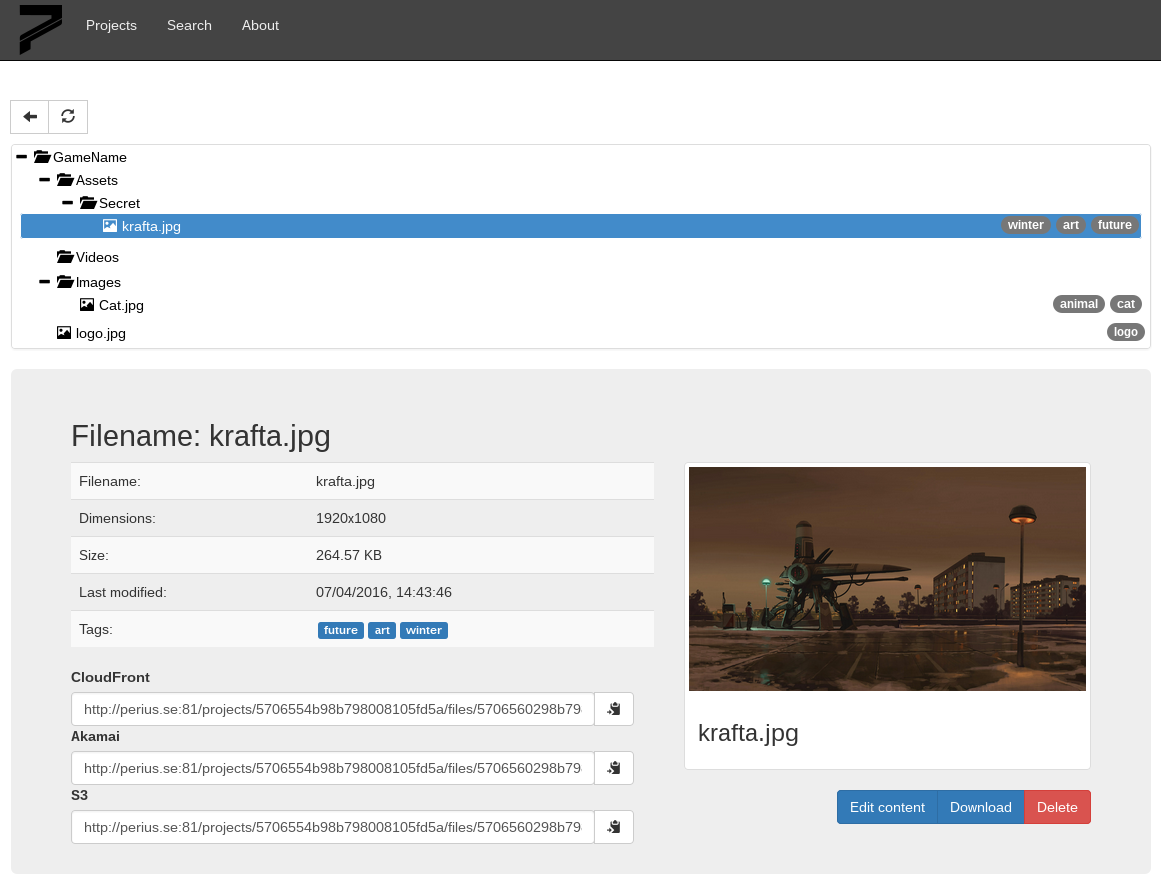
\includepdf[pages={1}]{front.pdf}
%\thispagestyle{empty}
%\newpage\null\thispagestyle{empty}\newpage

\pagenumbering{roman}
\setcounter{page}{1}

%\includepdf[pages={1}]{abstract.pdf}

%}}}
\begin{abstract}
    \fix Abstract

\keywords{}
\end{abstract}

%{{{
\newpage\null\thispagestyle{empty}\newpage

\setcounter{tocdepth}{3}
\tableofcontents

\clearpage
\pagenumbering{arabic}
\setcounter{page}{1}

%}}}
\section{Introduction}
Developing larger projects containing static content usually involves using a Content Distribution
Network to be able to scale to a large user base. The commercial Content Distribution Networks are
usually fairly easy to use, the content that is to be used in a project is usually simply uploaded
and then distributed over the globe when the public requests it. For secret content this can be a
problem and an inconvenience, and that is what this thesis is about. This work examines ways of
enforcing virtual access control on content and groups of content, in the form of folders and
snapshots. A system was developed to make the underlying theory work in practice. 

The research question that this report answers is how and whether it is practically feasible to use
Copy-on-Write for a high-level system like the one that is implemented. 

\fix Clarify problem definition and research questions

\subsection{Prior Work}
\subsubsection{Copy-on-Write}
This work relies heavily on the Copy-on-Write principle, which was founded and used in the Mach
kernel~\cite{COPYONWRITE}, as it can be used to efficiently create snapshots and help solving
concurrency problems that otherwise can occur.

Copy-on-Write is used in for example virtual memory management systems~\cite{VIRTCOW}, for snapshot
and as an optimisation technique for objects and types in several programming
languages\cite{LANGCOW}.

Its principle is that when processes or nodes share data in between each other, the data is not
copied until one of the processes does changes to it. This is an optimisation as the processes does
not have to send or copy all of the related data that is in memory, rather they only have to send
pointers to the data. After many Copy-on-Write's a complex tree structure can be built up, but
optimisations can be done to simplify that structure~\cite{COPYONWRITE2}.

\fix Polish and extend

\newpage
\section{Related Terminology}
\subsection{Abbreviations}
\subsubsection{JPF}
Java Path Finder - It was developed by NASA and in 2005 they released it under an open source
licence, which made more people contribute to the project. JPF is usually used for doing model
checking of concurrent programs to easily find for example race conditions and dead locks.

\subsubsection{CDN}
Content Distribution/Delivery Network - Replicates content to several servers, usually spread out
geographically. Once a request is made, the network serves content from the server closest to the
requester.

\subsection{Terms}
\subsubsection{Snapshot}
A snapshot is a way to record the full state of a system at a specific time. The term comes from
photography where a photo can be seen as the state of what the photo is of, at a certain time.
Snapshots should not be confused with full copies of a system as full copies can be used as backups
meanwhile snapshots are not very effective means of backups in the case of data corruption. It is
not effective against data corruption as snapshots usually still refer to unchanged data that is
still a part of the system~\cite{SNAPSHOT}.

\newpage 

\label{sec:model}
\section{Model}
The model for this work should show how the data can not be accessed or modified by unauthorized
users and how the integrity of the data is always kept in the Perius system. 

There could also be another relevant model done to show that content can not be accessed by
unauthorized viewers once the content is uploaded to a CDN, but as that should already have been
thoroughly checked by the CDN providers this work can focus solely on the internal users and content
of the management system. 

\subsection{Related work}

\subsection{Approach}

\subsection{Elements of the Model}
\fix Mathematical formal description of how the system works

\begin{center}
    \begin{tabular}{ | l | l | l | p{5cm} |}
        \hline
        Set & Elements & semantics \\ \hline
        C   & $c_0\dots c_n$                & Containers; folders in the virtual file system\\ \hline
        F   & $f_0\dots f_n$                & Files; files, images, videos\\ \hline
        P   & $p_0\dots p_n$                & Content; Meta-data for files\\ \hline
        U   & $u_0\dots u_n$                & Users; registered users in the system\\ \hline
        A   & $A[u_0,c_0]\dots A[u_n, c_n]$ & Access matrix; describes what containers users have access to\\ \hline
    \end{tabular}
\end{center}


\subsection{Access rights}
\begin{equation}
    \begin{split}
        u \in U \text{ can read } c \in C & \Iff u \in A[u,c] \\
        u \in U \text{ can write } c \in C & \Iff u \in A[u,c] \text{ and readonly } \notin c \\
        u \in U \text{ can delete } p \in c & \Iff u \in A[u,c] \text{ and readonly } \notin c \\
        u \nexists U \text{ can delete } f \in F \\
        \forall c \in C, \quad \exists u \in U & \mid a \in A[u,c] 
    \end{split}
\end{equation}

\subsection{Data integrity}
A computer system or subsystem is defined as possessing the property of integrity if it behaves consistently
according to a defined standard. This implies that a subsystem possessing the property of integrity
does not guarantee an absolute behaviour of the system, but rather that it performs according to
what its creator intended ~\cite{BIBA}.

\subsection{Initial Assumptions}
To create an integrity model, some initial assumptions have to be made about what the correct behaviour
of the system is, which the model then can be shown to follow. In this work unintentional behaviour
as the result of data modification is the main concern, which could be used for sabotage or simply be the
effect unintentional unfortunate race conditions etc. 

\subsection{Integrity Threats}
According to Biba et. al~\cite{BIBA} one can consider two threat sources, namely subsystem external
and subsystem internal. The external sources could be another system calling the subsystem with
faulty data or trying to make inaccurate calls to program functions, it could also be somebody
trying to tamper with the exposed functions of the program. Threats that are internal could be a
malicious part of the subsystem or simply an incorrect part of the subsystem, which does not behave
according to specification.

In this work external threats are handled as threats that can occur from what has been exposed by
the API (See Section~\ref{sec:API} and internal threats as incorrect implementation. As the server
and its system are assumed safe malicious subsystems are not considered.


\fix Translate to mathematical expressions

\begin{itemize}
    \item if a user wants to update a file in a content, the file is copied and the original is intact
    \item if a user reads content and then writes to it, the content is directly changed
    \item if a user copies content, a new content is created at the destination with reference to the same
          file
    \item if a user reads from a container and then writes to it, the container is directly changed
          (Which means last write wins, which doesn't matter)
    \item if a user creates a snapshot of a container, the full container tree is re created with 
          new ids at the destination, its content still refers to the same files.
\end{itemize}

\subsection{Findings}

\newpage
\section{Implementation}
\subsection{Background}
\subsubsection{About Uprise}
Uprise is a company based in Uppsala, Sweden. It is an EA studio focussing on creating great gaming
experiences, which means that they are not focussed on the actual gameplay which other EA studios
like DICE is. 

At the moment they are for example very involved with producing the Star Wars Battlefront game by
making menu systems and developing the companion app, Battlefront companion.

\subsubsection{The current system}
Today a system called battlebinary~\cite{BATTLEBINARY} is used for managing and uploading files,
mostly images, to content delivery networks. The current system does not make use out of the
security features that the CDN's are offering, instead it uses a form of security by obscurity. When
a file is uploaded to a CDN it is open for the public, but its filename is composed out of its
original filename concatenated with a part of the MD5 hash of the content of the file, which makes
it an extremely hard process to access the file on the CDN without access to the original file or a
reference to the URI.

In the current system you can only upload a file once as there will be a collision in the upload
otherwise, as the old and the new file will have the same MD5 hash.  

\subsubsection{Problem description}
As the current system does not offer proper security measurements, is lacking a lot of features that
is needed and does not scale very well, a new system should be developed. This work is about
examining a way of implementing Copy-on-Write in a high level system like this, which should solve
the scalability problem and make it possible to implement wanted features like snapshots, cloning
and concurrent modifications of content.

\subsection{Related Technologies}
\subsubsection{React}
React is a JavaScript library for building user interfaces. React uses both its own virtual DOM and
the browser's, this makes it able to efficiently update dynamic web pages after a change of state
through comparing the old virtual DOM with the resulting virtual DOM after the state change and then
only update the browser's DOM according to the delta between the virtual DOMs~\cite{REACT}. React
can be seen as the system for handling views in front-ends implementing a MVC
(Model-View-Controller) architecture.

\subsubsection{Reflux}
Reflux~\cite{REFLUX} is an idea and a simple library of how to structure your application. It
features a unidirectional dataflow (see Figure~\ref{fig:reflux}) which makes it more suitable, than
for example Flux~\cite{FLUX}, when using a functional reactive programming style.

\begin{figure}[htp] 
    \centering
    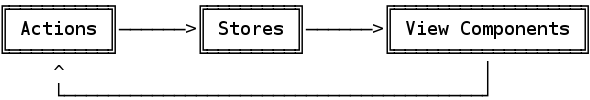
\includegraphics[scale=0.4]{reflux.png}
    \caption{Reflux unidirectional dataflow}
    \label{fig:reflux}
\end{figure}

\subsubsection{Scala} 
Scala is a multi-paradigm programming language. It most commonly runs on the JVM and compared to
Java it supports most functional programming features at the same time as it supports object
oriented programming~\cite{SCALA}.  

\subsubsection{REST} 
REST stands for representational state transfer, it is an architectural idea for writing stateless
services. These services usually use URIs to identify specific resources and HTTP to modify or query
these resources~\cite{REST}. 

\subsubsection{MongoDB}
MongoDB is a document-oriented database which means that it does not have the concept of rows as
normal relational databases has. Instead each entity in the database is stored as a document which
is not fixed to a predefined table structure~\cite{MONGODB}. MongoDB lacks support for joins too
improve its possibility to scale, which can be a big down side to some applications containing the
need for such logic.

\subsection{Methods for determining\\implementation details}
This chapter introduces the different methods used to determine how the new system should be
implemented, which DBMS it should use and how the estimation of long term scaling was done.

\subsection{Snapshot functionality}
\fix Structure to compare snapshot systems and conclude how Perius snapshot system was designed
\subsubsection{Copy-on-Write}
\label{sec:copy-on-write}
To efficiently create snapshots of a system Copy-on-Write can be used to make it possible to create
snapshots in O(1)\cite{BTRFS}, this is due to the fact that to create a snapshot in a system using
Copy-on-Write you only need to reference the current nodes in the tree and make sure that they are
not removed, see Figure~\ref{fig:btrfs_tree}.

As the persistent storage, used in this implementation (Section~\ref{persistent_storage}), does not
implement transactions or locks a lot of different problems can occur when several clients are
working on the same data set at the same time. Such problems could be race conditions and
determining the happened-before relation. In this work this problem is solved by implementing
Copy-on-Write.
\fix Move last paragraph

\subsubsection{Full Copy}
Full copy or deep copy, as opposed to copy-on-write, is a copy where everything is copied directly
and not only when an object is changed. This is easier to implement but is in most cases more
inefficient as more disk space will have to be used and if used with for example certain tree 
structures the part of the tree that needs to be copied will have to be traversed. 

\subsubsection{Comparison of Copy-on-Write system implementations}
\subsubsubsection{BTRFS}
Btrfs is a B-tree file system for Linux which makes use of Copy-on-Write to make it able to do
efficient writeable snapshots and clones. It also supports cloning of subtrees without having to
actually copy the whole subtree, this is due to the Copy-on-Write effect. As several nodes in the
tree can refer to the same node each node keeps track of how many parents it has by a reference
counter so that the node can be deallocated once the node does not have any parents any more. The
reference counter is not stored in the nodes themselves but rather in a separate data structure so
that a nodes counter can be modified without modifying the node itself and therefore eludes the
Copy-on-Write that would have to occur.

\begin{figure}[htp] \centering{
    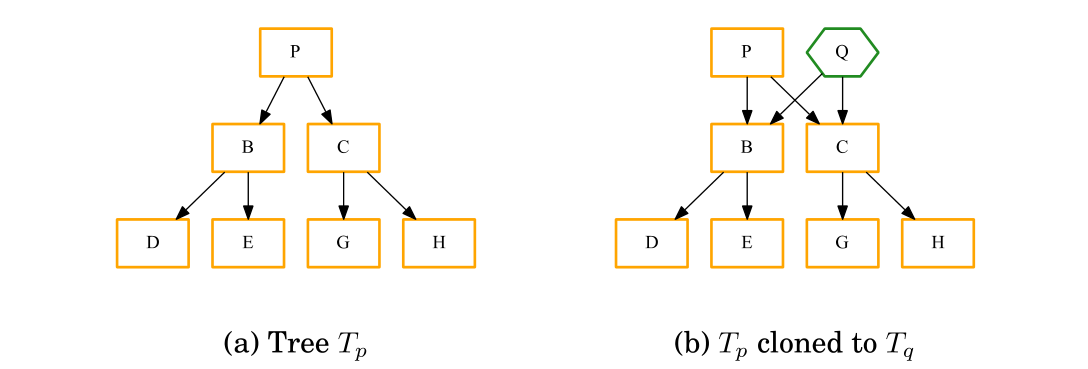
\includegraphics[scale=0.4]{newtree.png}}
    \caption{Cloning mechanism of Btrfs~\cite{BTRFS}}
    \label{fig:btrfs_tree}
\end{figure}

\subsubsubsection{Mach kernel}
In the mid 80's when the development of the Mach kernel started, there was problems with that
physically copying memory was too slow. Too minimise the copying of memory, Copy-on-Write was
implemented. It was implemented so that virtual copy operations could be done and so that tasks
could share read-write memory~\cite{MACH}.


\fix Insert more systems here

\subsubsection{Snapshot functionality of Perius}
In Perius snapshots and clones are not taken in the fashion which Btrfs uses, which can be seen in
Figure~\ref{fig:btrfs_tree}. As Perius does not have the tree structure pre-built and each node is
instead stored in a flat storage space, such operation would be too computationally expensive as
trees would have to be merged when collisions occur, due to the non-blocking nature of the
application. Instead this implementation makes a full copy of the meta-data of the tree, but still
refers to the same binary files until they are changed, which results in the creation of a new node.

\fix Relate section more to comparison

\subsection{Resulting system}
\subsubsection{Perius}
Perius is the implementation that was done to solve the problem at hand at Uprise. Perius has a
back-end written in Scala and a front-end written in ES6 (Javascript), but they are both
interchangeable.  The back-end has a REST API running, which is how the front-end communicates with
the back-end.

\fix Picture of the newest front-end
\begin{figure}[htp] \centering{
    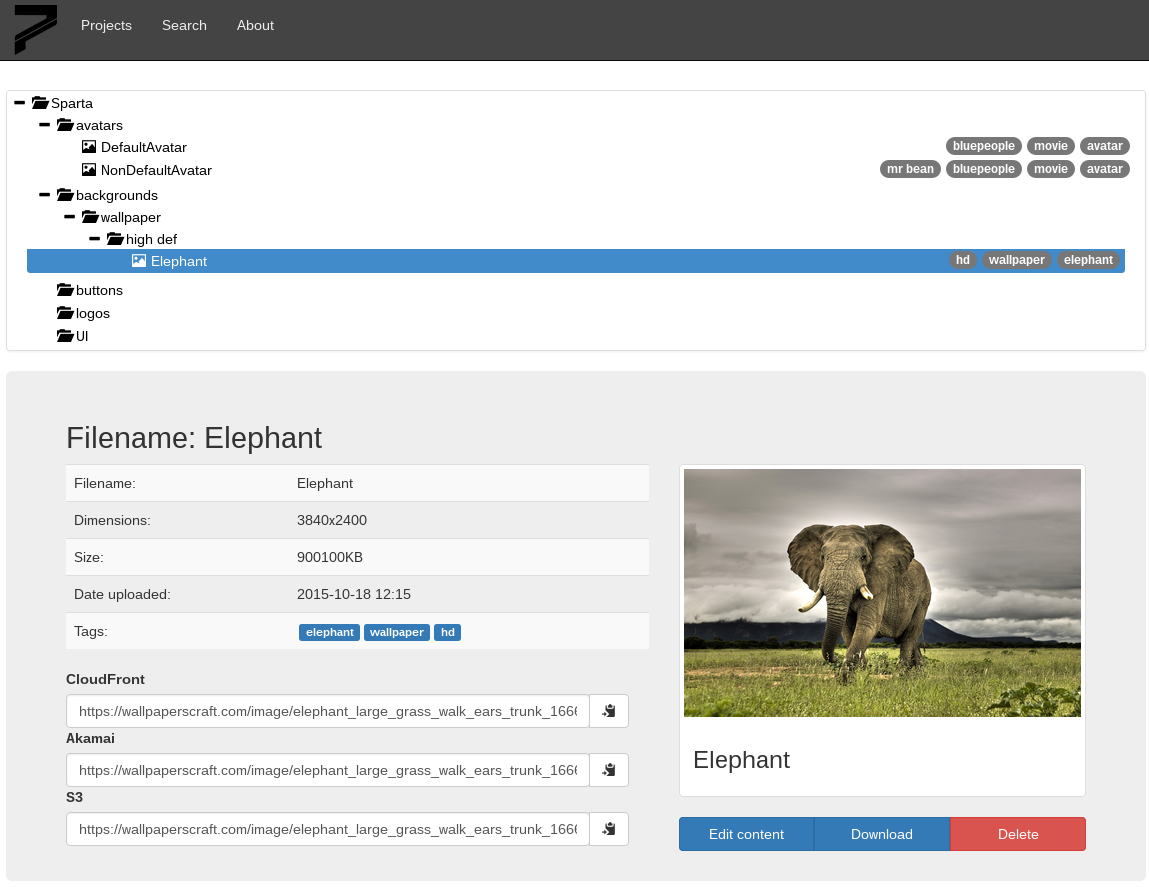
\includegraphics[scale=0.4]{frontend.png}}
    \caption{Front-end~\cite{BTRFS}}
    \label{fig:frontend}
\end{figure}


The service features a virtual file structure over the assets that has been stored, snapshots,
security management of whole containers as well as individual files, audit and access logging, multi
project support and a modular design for persistent storage.

The front-end is written in ES6 with React and Reflux, and the styling is done with the help of
Bootstrap.

\subsubsection{Copy-on-Write}
\fix Rename section and move

This implementation is far from as efficient as the other Copy-on-Write systems described in
Section~\ref{sec:copy-on-write} in most aspects, but more efficient in some. As the implementation
is built upon MongoDB as persistent storage and not a pure tree structure, single nodes can be
fetched in O(1) but when querying for subtrees they need to be built first, which takes O(log(n)),
where n is the number of nodes in the subtree. 

\subsubsection{Persistent storage}
\label{persistent_storage}
\subsubsubsection{MongoDB}
MongoDB was chosen as the persistent storage because of its quick lookups and because of its
internal storage format called BSON, which is very similar to JSON which the API is using. As the
formats are similar, the process of marshalling and unmarshalling becomes quite easy between the
core code, MongoDB instance and REST interface.  The second reason was that if the system needs to
scale in the future it is very easy to distribute MongoDB and if needed the system can easily be
migrated to Reactive Mongo, which is an asynchronous and non-blocking driver for MongoDB and can
therefore make the system scale even further~\cite{REACTIVEMONGO}.

\subsubsubsection{API}
\label{sec:API}
In this work a RESTful API was implemented and used for back-end $\Iff$ front-end
communication.

REST was chosen as only basic CRUD operations needs to be performed and because the BSON format
which is used in MongoDB is almost identical ~\cite{BSON} to the standardised JSON format which is
used by RESTful services~\cite{JSON}. 

\subsubsection{REST Endpoints}
For the front-end to communicate with the back-end, a RESTful service is implemented.
The following endpoints were configured:

\begin{itemize}
  \item projects
      \subitem GET - list all projects
      \subitem POST - create new project
  \item projects/\{id\}
      \subitem GET - get specific project
      \subitem PUT - update existing project
      \subitem DELETE - delete existing project
  \item projects/\{id\}/content
      \subitem POST - create new content in a specific project 
  \item projects/\{id\}/content/\{id\}
      \subitem GET - get specific content in a specific project
      \subitem PUT - update existing content in a specific project
      \subitem DELETE - delete existing content in a specific project

  \item projects/\{id\}/snapshots
      \subitem POST - create new snapshot in a specific project 

  \item projects/\{id\}/containers
      \subitem POST - create new container in a specific project 
  \item projects/\{id\}/containers/\{id\}
      \subitem GET - get specific container in a specific project
      \subitem PUT - update existing container
      \subitem DELETE - delete existing container
\end{itemize}

As can be seen several expected endpoints are missing, this is intentional as the operations missing
can be performed in a more efficient way. Such endpoint is for example \textit{GET 
projects/\{id\}/containers} as all containers exist in \textit{GET projects/\{id\}} and the interface
should present a file structure where both content and containers are shown.

\subsection{Findings}
\subsubsection{Scalability}

\subsubsection{Security of the system}
\paragraph{Authorization}
The authorization of the system is currently being handled by LDAP

\paragraph{Audit logs}


\section{JPF}
\fix Not sure where to put this section
JPF was used to test the idea and state transitioning of the application. Its a very simplified
version of the real system that still contains all the important Copy-on-Write core concepts and the 
assumptions that have been made for the model. This simplified version could then be automatically
tested for soundness. It is not a proof that the model works, but it is very exhaustive in its
testing.

\subsection{Entities}
\begin{figure}[htp] \centering{
    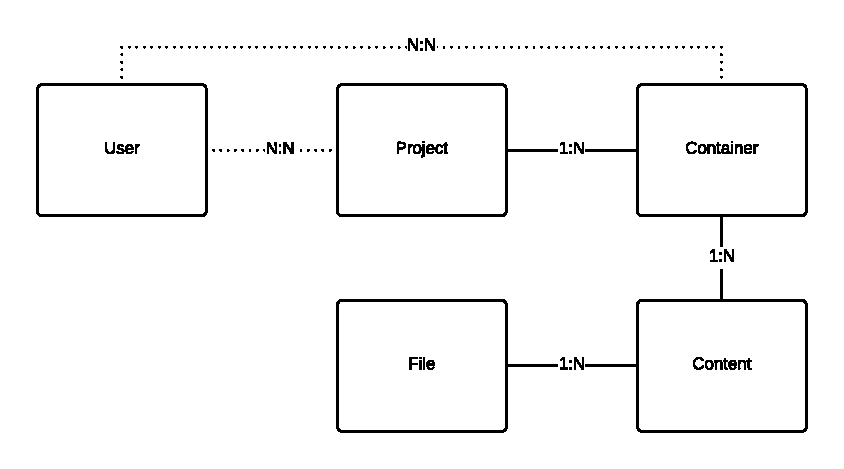
\includegraphics[scale=0.8]{relation.pdf}}
    \caption{High Level Entity Relationships}
    \label{fig:relation}
\end{figure}

\subsubsection{Content}
Content is meta data about a file and is stored in a container, it is a form of virtual file.  The
content can refer to for example an image, video or binary blob.

\subsubsection{Project}
A project is what is created to contain all content and containers related to a real project. Files
can be changed within a project and the system can contain several projects and their virtual
content are completely disjoint.

\subsubsection{Container}
A container is a virtual folder within a project which can contain content and other containers.

\subsubsection{Snapshot}
A snapshot is a read-only container from the state which the container the was in when the snapshot
was created.  A snapshot can not be updated and can only be deleted from the root of the snapshot.
Snapshots are by default stored as siblings to the container which they were made from, but they can
be contained by any container.

\subsubsection{File}
A file refers to an actual physical file. Files are stored in the database to make backup,
deployment and migration easier.

\subsubsection{User}
A user is the structure that handles people who have been granted access to the system. Access to
the system is handled by a separate service, like LDAP.

\subsection{Execution}
Java path finder was used to show that the model and plan of how to build the system was sound. The
model was built in Java with the objective of being as reduced and simple as possible, without
loosing any of the cases that needed to be covered by the model checker. As the users are mainly
going to be handled by external systems they were not included in the model.

Each collection in the persistent storage was emulated by using the built-in ConcurrentHashMap type.
Each client was represented by a thread and each action taken by the client was randomised. The id
hashes which MongoDB is using for each entity was imported from the mongo-java-driver-2.13.3 and
each object had its own id, generated in the same fashion as the real implementation is using,
randomly generated by the ObjectId class to minimise collisions that is.  Furthermore no locking or
transactions were used and the threads were running fully concurrently, without any sleep
statements. 

ConcurrentHashMap had to be used in instead of the normal HashMap, as the normal HashMaps can't be
iterated over concurrently.

JPF checked each permutation of states that the threads can end up in, the result of the run can be
seen in Listing~\ref{JPFRESULT}.

\begin{lstlisting}[label=JPFRESULT,caption=Results of JPF run]
elapsed time:       14:26:53
states:             new=160853259,
                    visited=451102505,
                    backtracked=611955764,
                    end=21640
search:             maxDepth=380,
                    constraints=0
choice generators:  thread=160853255 
                    (signal=0,
                    lock=3603938,
                    sharedRef=146989208,
                    threadApi=3,
                    reschedule=10260106), 
                    data=0

heap:               new=676056850,
                    released=435060996,
                    maxLive=655,
                    gcCycles=523950061

instructions:       11917045758
max memory:         6256MB
loaded code:        classes=111,
                    methods=2179
\end{lstlisting}


\section{Discussion}

\section{Summary}
\subsection{Conclusions}

\subsection{Future work}
Full access control was not implemented according to the model described in ~\ref{sec:model}, it
was only implemented to check whether a user should have access to the system as a whole or not, the
implementation did not set or check any specific access rights to certain contents or containers.



\newpage
\bibliographystyle{ieeetr}
\bibliography{references}

\end{document}


%{{{

%What to write about
%Battle Binary
%Security features of CDN's
%What is needed by the logic, like what happens after two consecutive deletes
%
%What is needed
%* Security layers
%* snapshots
%* Virtual file structure
%* Versioning of content
%* Multi project support
%* Auth and audit logs
%* Users

%Stuff to write about:
%Modular design, every piece should be interchangeable
%LDAP - why it was used as standard AUTH

%Using copy-on-write as the sole update strategy has pros and cons. The upside is
%that it is simple to guarantee operation atomicity, and data-structure integrity. The
%downside is that performance relies on the ability to maintain large extents of free
%contiguous disk areas. In addition, random updates to a f i le tend to fragment it,
%destroying sequentiality. A good defragmentation algorithm is required; this is
%described in Section 5

%}}}
